\section{Methodology}
\label{sec:methodology}

\begin{figure}
    \centering
    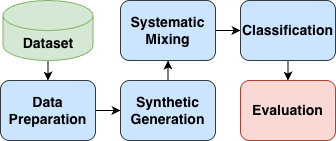
\includegraphics[width=1\linewidth]{pic/model_flowchart.png}
    \caption{Framework Flowchart}
    \label{fig:framework}
\end{figure}

Our methodology presents a systematic framework for rigorously evaluating LLM-generated synthetic spam data through large-scale replication and comprehensive statistical analysis. The framework addresses fundamental challenges in synthetic cybersecurity data assessment: quantifying quality-performance relationships, establishing statistical confidence in observed effects, and providing actionable guidance for operational deployment. As illustrated in Figure~\ref{fig:framework}, our approach integrates controlled generation, systematic mixing, and rigorous statistical evaluation to produce empirically grounded insights into synthetic data effectiveness.

\subsection{Framework Overview}

Our framework encompasses four primary stages that collectively enable rigorous assessment of synthetic spam data utility:

\begin{itemize}
\item \textbf{Stratified Data Preparation}: Systematic partitioning of real spam corpus into independent experimental groups using stratified random sampling, ensuring statistical independence while maintaining representation of diverse spam patterns across all groups.

\item \textbf{Controlled Synthetic Generation}: Application of multiple prompt engineering strategies to generate synthetic variants that systematically explore different aspects of spam semantic space, enabling controlled investigation of generation instruction impact on data quality.

\item \textbf{Systematic Mixing and Training}: Implementation of two fundamental mixing strategies (within-group and cross-group) across varying synthetic proportions, combined with multiple classifier architectures to comprehensively evaluate synthetic data utility under diverse conditions.

\item \textbf{Statistical Evaluation and Analysis}: Comprehensive assessment employing replicated measurements, hypothesis testing with multiple comparison correction, effect size quantification, and sensitivity analysis to establish statistically rigorous conclusions about synthetic data effectiveness.
\end{itemize}

This sequential approach ensures that each stage builds upon the previous one while maintaining clear separation of concerns, enabling systematic analysis of each component's contribution to overall synthetic data quality and utility.

\subsection{Theoretical Foundations and Design Rationale}

The framework is grounded in four fundamental principles that address key challenges in synthetic cybersecurity data evaluation.

\subsubsection{Statistical Replication for Robust Inference}

Our adoption of $R = 20$ independent experimental groups reflects statistical power analysis requirements for detecting practically meaningful effects. With 20 replications, we achieve statistical power exceeding 80\% for detecting medium effect sizes (Cohen's $d \geq 0.5$) at standard significance levels ($\alpha = 0.05$). This design choice transforms synthetic data evaluation from exploratory single-point estimation to rigorous hypothesis testing with quantified uncertainty, enabling confident conclusions about synthetic data effectiveness across operational variability.

The replication approach addresses a critical limitation in existing synthetic data research, where single-trial experiments cannot distinguish genuine treatment effects from random variation. By observing performance across 20 independent groups, we can quantify both central tendency (mean performance) and dispersion (standard deviation, confidence intervals), providing complete characterization of synthetic data impact rather than point estimates that may be unrepresentative.

\subsubsection{Controlled Prompt Engineering for Systematic Exploration}

The three-strategy prompt design (original, strong, weak) reflects our hypothesis that generation instructions systematically influence synthetic data characteristics along an intensity continuum. Rather than arbitrary prompt selection, we deliberately vary instruction emphasis on spam features to explore the generation parameter space systematically. This approach enables us to test whether explicit amplification of malicious characteristics (strong prompts) improves training utility compared to faithful reproduction (original) or subtle generation (weak prompts).

The controlled variation design follows principles from experimental psychology and human-computer interaction, where systematic manipulation of independent variables enables causal inference about their effects. By varying only prompt intensity while holding other factors constant, we isolate the contribution of generation instructions to downstream classifier performance.

\subsubsection{Distribution Matching Through Mixing Strategies}

Our within-group versus cross-group mixing strategies address fundamental questions about synthetic data generalization. The within-group strategy tests synthetic data effectiveness under ideal conditions where generated samples closely match the target training distribution, representing best-case scenarios where synthetic generation successfully captures local distributional characteristics.

The cross-group strategy deliberately introduces distributional mismatch by sourcing synthetic samples from different spam groups, testing whether synthetic data provides value through diversity and coverage rather than precise distribution matching. This design enables us to distinguish between two competing hypotheses about synthetic data mechanisms: (1) effectiveness requires close distribution matching, versus (2) effectiveness derives from semantic diversity that improves generalization. Real-world deployment often cannot guarantee precise distribution matching, making cross-group performance critical for assessing practical utility.

\subsubsection{Multi-Architecture Evaluation for Generalizability}

The inclusion of both Support Vector Machine (margin-based) and Random Forest (ensemble-based) classifiers addresses the concern that synthetic data effectiveness may be classifier-specific. Different classification architectures make fundamentally different assumptions about decision boundaries and data characteristics. SVMs construct optimal separating hyperplanes based on support vectors, potentially exhibiting sensitivity to distributional shifts in synthetic data. Random Forests aggregate multiple weak learners, potentially showing robustness to individual sample quality issues through ensemble averaging.

By evaluating synthetic data impact across architecturally distinct classifiers, we can distinguish between universal synthetic data properties and architecture-specific sensitivities, providing guidance for selecting appropriate classifiers when incorporating synthetic training data.

\subsection{Methodological Innovation}

The framework introduces several methodological innovations that advance the state of synthetic data evaluation in cybersecurity contexts.

\subsubsection{Large-Scale Replication for Statistical Rigor}

Our $R = 20$ replication design represents, to our knowledge, the first application of large-scale statistical replication to synthetic cybersecurity data evaluation. Prior work typically reports single-trial results or limited replication ($R \leq 5$), providing insufficient statistical power for confident inference. Our design enables:

\begin{itemize}
    \item \textbf{Hypothesis testing with multiplicity control}: Application of False Discovery Rate correction to control type I error inflation across multiple comparisons, ensuring reported significant effects are unlikely to be spurious.

    \item \textbf{Effect size quantification}: Calculation of Cohen's $d$ effect sizes to distinguish between statistically significant but practically negligible effects versus substantial impacts that warrant operational consideration.

    \item \textbf{Confidence interval estimation}: Precise quantification of uncertainty in performance estimates, enabling risk-aware decision making about synthetic data deployment.

    \item \textbf{Sensitivity analysis}: Regression modeling of performance as a function of synthetic proportion, quantifying degradation rates and enabling performance prediction for arbitrary mixing ratios.
\end{itemize}

\subsubsection{Systematic Mixing Strategy Investigation}

The explicit comparison of within-group versus cross-group mixing strategies addresses a gap in existing research, which typically employs a single mixing approach without investigating alternatives. Our systematic investigation enables empirical answers to critical deployment questions: Can synthetic data from one source effectively augment training data from another source? Does precise distribution matching matter, or is semantic diversity sufficient? These questions directly impact operational decisions about synthetic data sourcing, transfer learning, and temporal adaptation.

\subsubsection{Comprehensive Performance Degradation Characterization}

Our sensitivity analysis framework, modeling classifier performance as a function of synthetic proportion through linear regression, provides quantitative degradation metrics that enable cost-benefit analysis. The regression slope ($\beta_1$) quantifies expected performance change per percentage point increase in synthetic data, while $R^2$ indicates whether degradation patterns are linear (enabling simple prediction) or non-linear (requiring more complex modeling). This framework transforms qualitative observations about synthetic data impact into quantitative relationships suitable for operational decision support.

\subsection{Evaluation Metrics Framework}

Our methodology employs a comprehensive metrics suite that captures synthetic data effectiveness from multiple perspectives, enabling both immediate performance assessment and long-term optimization guidance.

\subsubsection{Classification Performance Metrics}

The classification metrics provide standard machine learning assessment across all experimental conditions, ensuring comprehensive evaluation of synthetic data utility for operational spam detection:

\begin{itemize}
\item \textbf{Accuracy}: Overall correctness rate measuring the proportion of correctly classified samples. While informative, accuracy can be misleading under class imbalance, motivating our emphasis on additional metrics.

\item \textbf{Precision}: True positive rate for spam detection, quantifying the reliability of positive classifications. High precision minimizes false positives, critical for maintaining user trust in spam filtering systems.

\item \textbf{Recall}: Sensitivity measure capturing the ability to identify spam samples. High recall minimizes false negatives, ensuring that malicious content is reliably detected.

\item \textbf{F1-Score}: Harmonic mean of precision and recall, providing balanced assessment particularly important under class imbalance conditions. The F1-score serves as our primary metric for comparing synthetic data strategies, as it equally weights both error types.

\item \textbf{AUC-ROC}: Area under the receiver operating characteristic curve, measuring classifier discrimination ability across all decision thresholds. AUC-ROC provides threshold-independent assessment, complementing threshold-dependent metrics.

\item \textbf{Specificity}: True negative rate for legitimate email detection, quantifying the ability to correctly identify benign samples. High specificity minimizes legitimate email misclassification.

\item \textbf{Matthews Correlation Coefficient (MCC)}: Balanced measure considering all confusion matrix elements, providing robust performance assessment even under severe class imbalance.
\end{itemize}

\subsubsection{Statistical Analysis Metrics}

Beyond classification performance, our framework employs rigorous statistical metrics to quantify confidence, effect magnitude, and degradation patterns:

\begin{itemize}
\item \textbf{Descriptive Statistics}: For each configuration, we compute mean and standard deviation across $R = 20$ replications:
\begin{equation}
\bar{m} = \frac{1}{R}\sum_{r=1}^{R} m_r, \qquad
s_m = \sqrt{\frac{1}{R-1}\sum_{r=1}^{R} (m_r - \bar{m})^2}
\end{equation}
where $m_r$ denotes the performance metric for the $r$-th experimental group. The mean $\bar{m}$ quantifies expected performance, while standard deviation $s_m$ indicates consistency across operational variability. This replicated measurement approach provides complete distributional characterization rather than single-point estimates.

\item \textbf{Confidence Intervals}: 95\% confidence intervals quantify estimation uncertainty for all performance metrics:
\begin{equation}
\text{CI}_{95\%} \approx \bar{m} \pm 1.96 \cdot \frac{s_m}{\sqrt{R}}
\end{equation}
For $R = 20$ replications, this yields margin of error $\approx 0.44 \cdot s_m$, providing reasonable precision for operational decision making. Narrow intervals indicate precise estimates, while wide intervals suggest high variability requiring cautious interpretation. Complete t-distribution formulation accounting for finite sample size is provided in Appendix~\ref{appendix:statistics}.

\item \textbf{Hypothesis Testing}: Paired t-tests comparing each synthetic ratio against baseline (0\% synthetic), with Benjamini-Hochberg False Discovery Rate correction for multiple comparisons. This approach controls expected proportion of false discoveries while maintaining reasonable statistical power.

\item \textbf{Effect Sizes}: Cohen's $d$ quantifying standardized mean differences between conditions. Effect size interpretation follows standard guidelines: $|d| < 0.2$ = negligible, $0.2 \leq |d| < 0.5$ = small, $0.5 \leq |d| < 0.8$ = medium, $|d| \geq 0.8$ = large.

\item \textbf{Sensitivity Analysis}: Linear regression modeling performance as a function of synthetic proportion:
\[
\text{Performance} = \beta_0 + \beta_1 \cdot \theta + \epsilon
\]
where $\theta$ is synthetic proportion (0-100\%), $\beta_1$ is the degradation rate (slope), and $R^2$ quantifies linearity of the relationship. The slope provides a practical metric for operational planning: expected performance change per 1\% increase in synthetic data.
\end{itemize}

\subsection{Quality Assurance and Validation}

Our methodology incorporates multiple quality assurance mechanisms to ensure reliable and reproducible results.

\subsubsection{Sampling Quality Control}

The stratified sampling approach guarantees that each of the 20 groups maintains consistent class distribution (10\% spam) while representing diverse spam patterns. Sampling without replacement ensures group independence, enabling valid application of parametric statistical tests. Post-sampling validation confirms that spam characteristics (e.g., content length, keyword distributions) remain balanced across groups, preventing confounding between group assignment and spam type.

\subsubsection{Generation Quality Verification}

All LLM-generated synthetic samples undergo validation to ensure successful generation and parsability. Failed generations or malformed outputs are logged and excluded from analysis, with generation success rates reported for transparency. This approach ensures that observed performance differences reflect genuine synthetic data quality rather than parsing failures or incomplete samples.

\subsubsection{Experimental Reproducibility}

The framework emphasizes reproducibility through comprehensive documentation and controlled randomization:

\begin{itemize}
    \item \textbf{Fixed Random Seeds}: All random processes (sampling, train-test split, model initialization) employ fixed seeds documented in experimental records, enabling exact replication of results.

    \item \textbf{Consistent Test Set}: A single fixed out-of-sample test set is used across all 1,320 experimental conditions (3 prompts $\times$ 2 strategies $\times$ 11 ratios $\times$ 20 groups), eliminating test set variance as a confounding factor.

    \item \textbf{Hyperparameter Standardization}: Classifier hyperparameters remain constant across all experiments, isolating synthetic data impact from model configuration effects.

    \item \textbf{Version Control}: All code, prompts, and analysis scripts are version controlled and archived, enabling future replication and extension.
\end{itemize}

\subsubsection{Statistical Validity}

Our statistical analysis adheres to best practices for multiple comparison correction, assumption verification, and robust estimation:

\begin{itemize}
    \item \textbf{Assumption Testing}: Normality assumptions for parametric tests are verified using Shapiro-Wilk tests. When violated, we employ non-parametric alternatives (Wilcoxon signed-rank tests) and bootstrap confidence intervals for robust inference.

    \item \textbf{Multiple Comparison Correction}: The Benjamini-Hochberg False Discovery Rate procedure controls the expected proportion of false discoveries across 11 synthetic ratios $\times$ 2 classifiers $\times$ 7 metrics = 154 hypothesis tests per configuration, preventing spurious significance claims.

    \item \textbf{Effect Size Reporting}: All significant effects are accompanied by effect size measures (Cohen's $d$), enabling readers to distinguish between statistically significant but trivial effects versus substantial impacts warranting practical consideration.
\end{itemize}

\subsection{Methodological Limitations and Scope}

While our framework provides rigorous evaluation of synthetic spam data, several limitations define the scope of our conclusions:

\begin{itemize}
    \item \textbf{Feature Representation}: Our evaluation employs TF-IDF feature representation, which captures lexical patterns but may miss deeper semantic or structural characteristics. Deep learning classifiers operating on embeddings might exhibit different sensitivity profiles.

    \item \textbf{Dataset Specificity}: Results are based on the CEAS-08 spam corpus, which represents spam patterns from a specific time period and threat landscape. Generalization to other spam datasets or evolving spam tactics requires empirical validation.

    \item \textbf{Class Imbalance Range}: Our fixed 10\% spam ratio reflects common operational conditions but does not explore the full spectrum of possible imbalance scenarios. More extreme imbalances may exhibit different synthetic data effectiveness patterns.

    \item \textbf{LLM Selection}: We employ GPT-4.1-mini as our generation engine. Different LLMs with varying capabilities may produce synthetic data with different quality characteristics and performance impacts.
\end{itemize}

These limitations define boundary conditions for our findings and suggest directions for future research extending the framework to additional datasets, classifiers, and generation models.

\subsection{Methodological Contributions}

By integrating large-scale replication, systematic prompt engineering, controlled mixing strategies, and comprehensive statistical analysis, our methodology establishes a rigorous framework for synthetic cybersecurity data evaluation. The framework's emphasis on statistical power, effect size quantification, and degradation characterization moves synthetic data research beyond exploratory single-trial evaluations toward confirmatory hypothesis testing with quantified uncertainty.

This methodological foundation enables evidence-based decision making about synthetic data deployment in operational cybersecurity systems, providing practitioners with quantitative guidance for selecting generation strategies, choosing mixing ratios, and predicting performance impacts. The framework's modular design facilitates adaptation to other cybersecurity domains beyond spam detection, potentially advancing synthetic data research across malware analysis, intrusion detection, and threat intelligence applications.
